\documentclass[11pt]{beamer}

\usecolortheme{rose} % Layout-Definitionen
\useinnertheme[shadow]{rounded} % Layout-Definitionen

\usepackage[ngerman]{babel} % neue deutsche Rechtschreibung
\usepackage[T1]{fontenc} % vortragstaugliche Schrift
\usepackage{lmodern} % vortragstaugliche Schrift
\usepackage{tikz}
\usepackage{amsfonts}
\usepackage{graphicx}
\usepackage[cspex,bbgreekl]{mathbbol}
\usepackage{aligned-overset}
\usetikzlibrary{graphs}

\graphicspath{ {./images/} }

\title{Der Kontaktprozess} 
\author{Lukas Koebe}
\institute{Technische Universit\"at M\"unchen}
\date{\today}

\begin{document}

% Titelseite:
\begin{frame}
\titlepage
\end{frame}

\setbeamercovered{dynamic}
\begin{frame}
\frametitle{Kontaktprozess}
Sei $G = (V, E)$ ein zusammenhängender Graph mit endlichem Grad
($\forall v \in V : |\{ e \in E | \exists u \in V : e = \{v, u\} \}| < \infty$).
\begin{itemize}
    \item Wir betrachten die Knoten als Individuen
    \item Die Individuen können von einer Krankheit infiziert werden
    \item Wir betrachten einen stochastischen Prozess in kontinuierlicher Zeit
\end{itemize}
\end{frame}


\begin{frame}{Kontaktprozess}
Wir definieren den Zustandsraum $\Sigma = \{ 0, 1 \}^V$ als die Menge aller Zustände.
\begin{itemize}
    \item Zustand 1 entspricht krankem Individuum
    \item Zustand 0 entspricht gesundem Individuum
\end{itemize}
Für jeden Zeitpunkt $t \in [0, \infty)$ definiere $\xi_t \in \Sigma$ als
den Zustand der Individuen zum Zeitpunkt $t$.
\\
Das bedeutet: ist $\xi_t(x) = 1$, so ist das Individuum $x$ zum Zeitpunkt $t$ infiziert.
\end{frame}

\begin{frame}{Modellierung der Verbreitung}
    Wenn eine Kante zwischen zwei Knoten existiert, kennen sich die beiden Individuen,
    bzw. können einander infizieren.
    \begin{itemize}
        \item[(i)]<2-> 
            Wenn ein Individuum $x$ infiziert ist, kann es alle gesunden Individuen in seiner Nachbarschaft
            \begin{equation*}
                N(x) = \{ y \in V | \exists e \in E : {x, y} \in E \}
            \end{equation*}
            mit einer Ansteckungsrate $\beta \geq 0$ anstecken.
        \item[(ii)]<3->
            Die Wartezeit dafür exponentiell verteilt, mit Erwartungswert $\frac{1}{\beta}$. (mehr später) 
        \item[(iii)]
            höheres $\beta$ impliziert schnellere Wiederholung
        \item[(iv)]<4-> 
            Infizierte Individuen werden mit einer Rate $\delta \geq 0$ spontan wieder
            gesund. (durchschnittliche Zeit bis zur genesung $\frac{1}{\delta}$)
    \end{itemize}
    \onslide<2> {
    }
\end{frame}

\begin{frame}{Markow-Eigenschaft für endliche Graphen}
    Kontaktprozess ist ein Markow Prozess für endliche Graphen, da:
    \[
        \mathbb{P}(\xi_{t + h} \in A\ |\ \xi_{t}) = \mathbb{P}(\xi_{t + h} \in A\ |\ \{ \xi_s\ s \leq t \})
    \]
\end{frame}
% Auf unendlichen Graphen ist es nicht klar ersichtlich, ob der Kontaktprozess
% wohldefiniert ist, da die Zustandsmenge $\Sigma$ überabzählbar unendlich ist.

\begin{frame}{Poisson-Punkt-Prozess}
    Modellierung zufälliger, voneinander unabhängig auftretender Ereignisse
    \begin{itemize}
        \item $X_i, i \geq 1, X_i \sim exp(\beta)$ unabhängig
        \item $S_n = \sum_{i = 1}^n X_i$
        \item $\eta = \sum_{n = 1}^\infty \delta_{S_n}$ ist Poisson Prozess
        \item wir schreiben oft $\eta$ statt $\{x \in [0, \infty)\ |\ \eta(x) \not= 0 \}$
    \end{itemize}
\end{frame}
\begin{frame}
    Eigenschaften des Poisson-Punkt-Prozesses:
    \begin{itemize}
        \item [(i)]<2-> Für $B \subseteq [0, \infty)$ ist $|\eta(B)| \sim Poisson(\beta \cdot \bblambda(B))$  
        \item [(ii)]<3-> Für paarweise Disjunkte Mengen $B_1$, $B_2$, $B_3$, ..., $B_n \subseteq [0, \infty)$ 
        sind $\eta(B_1), \eta(B_2), \eta(B_3), ..., \eta(B_n)$ unabhängig.
        \item [(iii)]<4-> $\eta_1 + \eta_2 \sim Poisson(\beta_1 + \beta_2)$, für
        $\eta_1 \in Poisson(\beta_1)$ und $\eta_2 \in Poisson(\beta_2)$
        (Superpositionseigenschaft)
        \item [(iv)]<5-> Entfernen von Punkten aus $\eta$ mit Wahrscheinlichkeit $1 - p$ ergibt einen Prozess $\eta^\prime \sim Poisson(p \cdot \beta)$ (Ausdünnungseigenschaft)
    \end{itemize}
\end{frame}

%Konstruktion des Kontaktprozesses als eine abzählbare Menge von Poisson Punktprozessen,
    %sowie zusätzlich ein hilfreiches Werkzeug für Beweise mittels Kopplung.
    %Hier nur für Kontaktprozess gezeigt, funktioniert jedoch für verschiedene interagierende
    %stochastische Partikelsysteme.

\setbeamercovered{transparent}
\begin{frame}{Harris' graphische Darstellung}
Sei $G = (V, E)$ Graph mit endlichem Grad, (als Beispiel $\mathbb{L}^1$  in Grafik). Nun betrachten wir $G \times \mathbb{R}^+_0$. Wobei wir die reelle Halbachse
als Zeitachse betrachten.
\begin{center}
    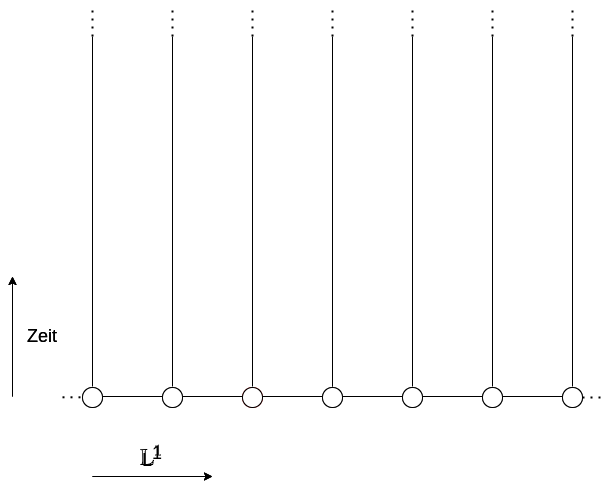
\includegraphics[width=0.75\textwidth]{images/contact process time.png}
\end{center}
\end{frame}

\begin{frame}{Harris' graphische Darstellung - Genesungsrate $\delta$}
    Für alle $x \in V$ seien $D_x$ ein Poisson-Punkt-Prozesse mit Parameter $\delta$ und unabhängig.
    \begin{itemize}
        \item $t \in D_x$ als Zeitpunkte spontaner Heilung
        \item In Harris' graphischer Darstellung zeichne ein Kreuz auf $(x, t)$ für jeden Punkt
            $t \in D_x$
    \end{itemize}
    \begin{center}
        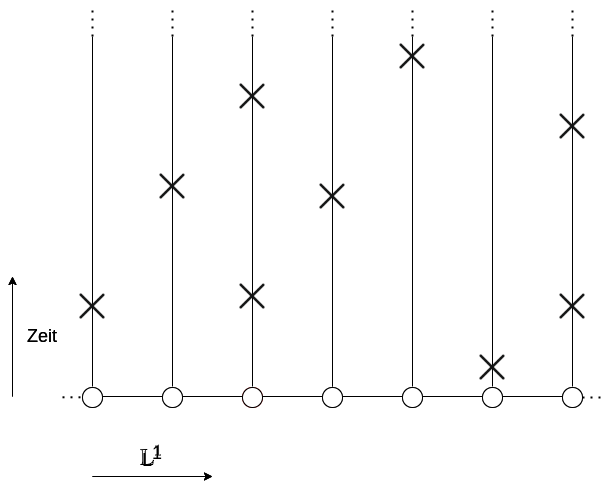
\includegraphics[width=0.6\textwidth]{images/contact process crosses.png}
    \end{center}
\end{frame}

\begin{frame}{Harris' graphische Darstellung - Infektionsrate $\beta$}
    Für jede Kante $e = \{ x, y \} \in E$ sei $B_{x, y}$ ein Poisson-Punkt-Prozess mit Parameter
    $\beta$.
    \begin{itemize}
        \item $t \in B_{x, y}$ als Zeitpunkte der Infektion von $y$ durch $x$
        \item In Harris' graphischer Darstellung durch einen Pfeil von $(x, t)$ nach $(y, t)$
        dargestellt
    \end{itemize}
    % falls das individuum x zum Zeitpunkt t überhaupt infiziert ist
    \begin{center}
        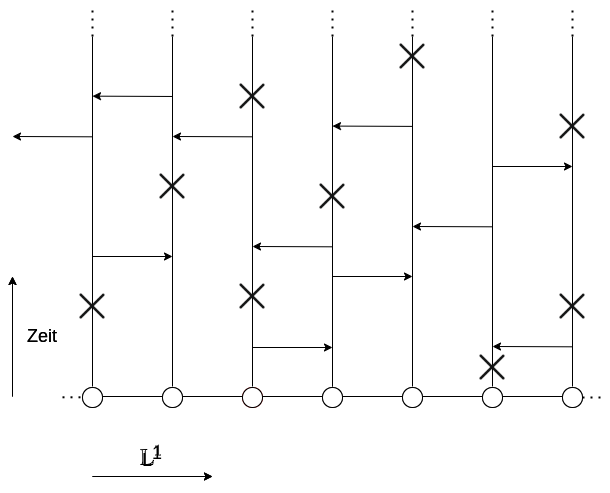
\includegraphics[width = 0.6\textwidth]{images/contact process arrows.png}
    \end{center}
\end{frame}

\begin{frame}{Harris' graphische Darstellung - Pfade}
    Für $t_0 < t_1 < ... < t_n < t_{n + 1}$ und $x_0, x_1, ..., x_n \in V$
    und $B_{x_i, x_{i + 1}} \cap [t_i, t_{i + 1}] = \emptyset$, sowie $t_i \in D_{x_{i - 1}}$ für
    $0 \leq i \leq n$, schreiben wir 
    \begin{equation*}
        (x, t) \to (y, s)
    \end{equation*}
    wenn $x = x_0, y = x_n$ und $t = t_0, s = t_{n + 1}$.
    \begin{center}
        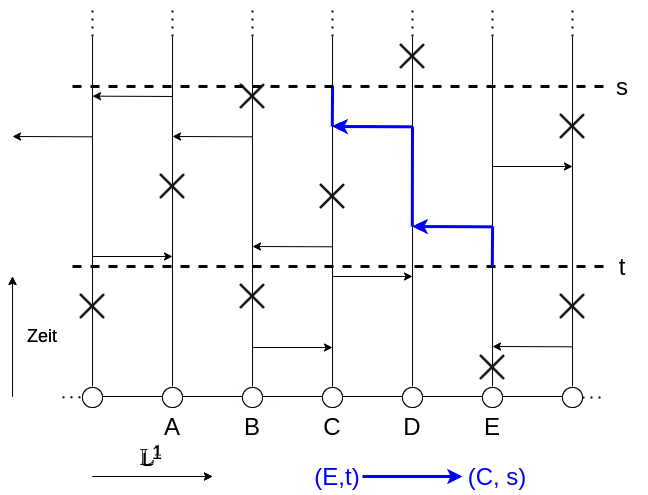
\includegraphics[width=0.6\textwidth]{images/contact process path.png}
    \end{center}
\end{frame}

\begin{frame}{Pfade - Infektionsweg}
    Sei $\xi_0 \in \Sigma = \{0, 1\}^V$ ein Anfangszustand. Wir definieren $\xi_t: V \to \Sigma$ für
    $x \in V, t \in \mathbb{R}^+_0$ als $\xi_t(x) := 1$ genau dann, wenn es
    einen Pfad von $(y, 0) \to (x, t)$ mit $y \in V$ gibt und $\xi_0(y) = 1$.
    \\
    Dann ist $\xi_t$ ein Kontaktprozess mit Infektionsrate $\beta$ und Heilungsrate $\delta$.
    % Intuitiv ist es klar, dass es sich bei $\xi_t$ um den oben definierten Kontaktprozess handelt.
    % Individuen können andere mit einer Rate von $\beta$ infizieren und mit einer Rate $\delta$
    % spontan genesen. Durch die Konstruktion (und insbesondere die Gedächtnislosigkeit der einzelnen
    % Poisson-Punkt-Prozesse) ist die Markow-Eigenschaft des Prozesses gegeben.
    \begin{center}
        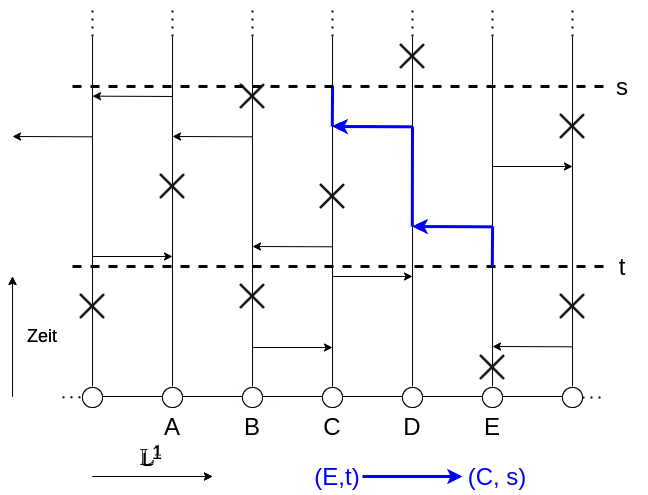
\includegraphics[width=0.6\textwidth]{images/contact process path.png}
    \end{center}
\end{frame}

\begin{frame}{Endliche Cluster}
    %Nun muss noch geklärt werden, ob es möglich ist, für einen Zeitpunkt $t$ den Zustand des
    %Prozesses in endlicher Zeit zu konstruieren. Dafür wollen wir zeigen, dass wir für eine
    %ausreichend kleine Zeit $\varepsilon > 0$ und einen gegebenen Zustand $\xi_s$ zum Zeitpunkt
    %$s$ in endlicher Zeit den Zustand $\xi_{s + \varepsilon}(x)$ eines Knoten $x \in V$ zum
    %Zeitpunkt $s + \varepsilon$ berechnen können.
    
    %Da es sich bei $\mathbb{L}^d$ um einen unendlichen Graphen handelt, ist es auf den ersten
    %Blick nicht eindeutig ersichtlich wie viele Knoten aus $\mathbb{L}^d$ einen Einfluss auf
    %den Knoten $x$ haben können.
    Sei $\xi_t$ eine Realisierung des Kontaktprozess mit Parametern $\beta, \delta > 0$.
    Dann sei 
    \begin{equation*}
        I_{x, t, t + \varepsilon} := \{y \in V\ |\ \exists s : t < s < t + \varepsilon \wedge (x,t) \to (y,s) \} 
        \end{equation*}
    die Menge der Knoten, mit einem Pfad der maximalen Länge
    $\varepsilon$ nach $x$ beginnend zum Zeitpunkt $t$. 
    \begin{block}{Lemma}
        Es gibt ein $\varepsilon > 0$, sodass für alle Knoten $x \in V$ gilt
        \begin{equation*}
            \mathbb{P}(\{ \#I_{x, t, t + \varepsilon} < \infty \}) = 1
        \end{equation*}
    \end{block}
\end{frame}

\begin{frame}{Einflussbereich}
    Wir definieren eine Kante $e = \{x_1, x_2\} \in E$ als offen im Zeitraum $[t, t + \varepsilon]$
    genau dann wenn $(B_{x_1, x_2} \cup B_{x_2, x_1}) \cap [t, t + \varepsilon] \not= \emptyset$
    
    \begin{block}{Lemma}
        $\mathbb{P}(\{ e\ \text{ist offen im Zeitraum}\ [t, t + \varepsilon] \}) = 1 - e^{-2\beta\varepsilon}$
    \end{block}
    \textbf{Beweis:}
    \begin{itemize}
        \item $|B_{x_1,x_2}| \sim Poisson(\beta)$
        \item Unabhängigkeit von $B_{x_1,x_2}$ und $B_{x_1,x_2}$
        \item $\mathbb{P}(|\eta([t, t + \varepsilon])| = 0) =  1 - e^{-2\beta\varepsilon}$
    \end{itemize}
    Wahrscheinlichkeit für $\{ e \text{ offen in}\ [t, t + \varepsilon] \} $ beliebig klein wählbar
\end{frame}

\begin{frame}{Einflussbereich}
    \begin{center}
        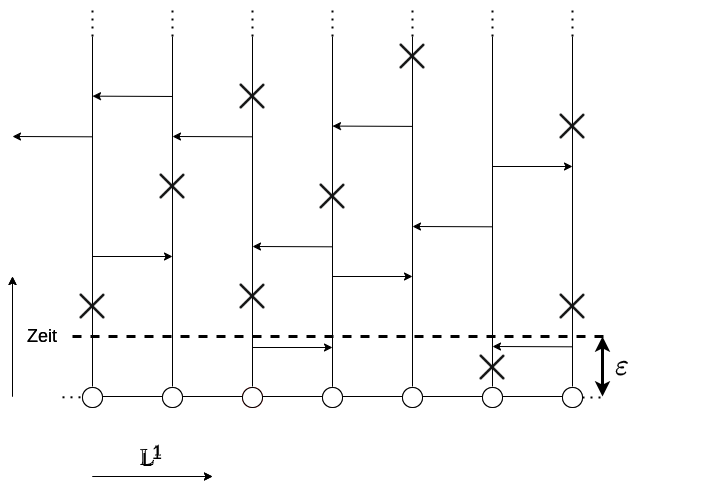
\includegraphics[width=0.75\textwidth]{images/contact process epsilon.png}
    \end{center}
\end{frame}

\setbeamercovered{dynamic}
\begin{frame}{Einflussbereich - Perkolation}
    Wir wissen, dass die kritische Wahrscheinlichkeit $p_c$ für Perkolationen
    auf $\mathbb{L}^D$ nicht degeneriert ist, also $0 < p_c < 1$.
    Und dass für alle $p < p_c$ die Perkolationswahrscheinlichkeit
    $\theta(p) = \mathbb{P}(|C_0| = \infty) = 0$.
    \onslide<2->
    \vspace{1cm}
    \\
    Es gibt also ein $\varepsilon > 0$, sodass die Perkolationswahrscheinlichkeit der
    offenen Kanten in $G$, $\theta(1 - e^{-2\beta\epsilon}) = 0$ ist.
\end{frame}

\begin{frame}{Einflussbereich}
    Aus der Konstruktion von $I_{x, t, t + \varepsilon}$ folgt, dass
    \begin{equation*}
        \{ |I_{x, t, t + \varepsilon}| < \infty \} \subseteq \{ |C_x| < \infty \}   
    \end{equation*}
    woraus wiederum folgt, dass
    \begin{equation*}
        \mathbb{P}(\{ |I_{x, t, t + \varepsilon}| < \infty \}) \leq \mathbb{P}(\{ |C_x| < \infty \}) = 1
    \end{equation*}
    und damit auch das oben genannte Lemma.
    \\
    Es genügt die Betrachtung einer endlichen Anzahl von Knoten zum Zeitpunkt $t$ zur Bestimmung
    von $\xi_{t + \varepsilon}(x)$ zum Zeitpunkt $t + \varepsilon$
\end{frame}

\begin{frame}{Harris' graphische Darstellung - Kopplung}
    Seien $\beta_1 \leq \beta_2$ und $\delta_1 \geq \delta_2$. Wir betrachten nun
    eine Realisierung eines Kontaktprozesses mit Parametern $(\beta_2, \delta_1)$.
    \begin{itemize}
        \item<2-> Wir entfernen zufällig Punkte aus $B_{x, y}$ (Pfeile) mit Wahrscheinlichkeit
        $1 - \frac{\beta_1}{\beta_2}$.
        \item<3-> Kontaktprozess mit Parametern $(\beta_1, \delta_1)$ (Ausdünnungseigenschaft)
        \item<4-> Höchstens gleich viele Infektionen bei selbem Ausgangszustand
    \end{itemize}
    \onslide<5->
    $\implies$ \#Infektionen nicht-fallend mit Infektionsrate $\beta$
\end{frame}

\begin{frame}{Harris' graphische Darstellung - nicht wachsend in $\beta$}
    \begin{center}
        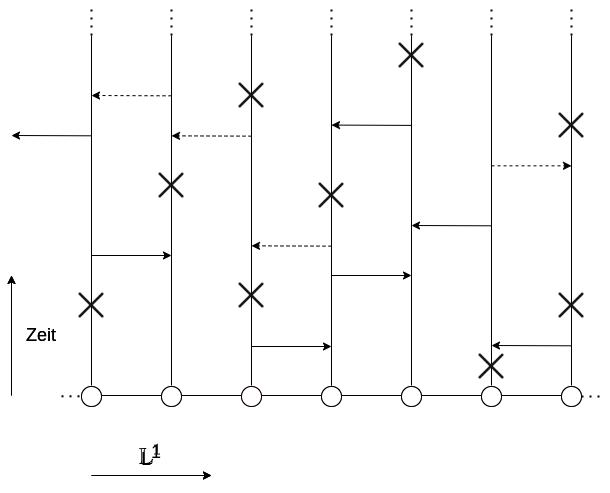
\includegraphics[width=0.75\textwidth]{images/contact process dotted arrows.png}
    \end{center}
\end{frame}

\begin{frame}{Harris' graphische Darstellung - Kopplung}
    Seien $\beta_1 \leq \beta_2$ und $\delta_1 \geq \delta_2$. Wir betrachten nun
    eine Realisierung eines Kontaktprozesses mit Parametern $(\beta_2, \delta_1)$.
    \begin{itemize}
        \item<2-> Wir entfernen zufällig Punkte aus $D_x$ (Kreuze) mit Wahrscheinlichkeit
        $1 - \frac{\delta_2}{\delta_1}$.
        \item<3-> Kontaktprozess mit Parametern $(\beta_2, \delta_2)$ (Ausdünnungseigenschaft)
        \item<4-> Mindestens gleich viele Infektionen bei gleichem Ausgangszustand
    \end{itemize}
    \onslide<5->
    $\implies$ \#Infektionen nicht-fallend mit Heilungsrate $\delta$
\end{frame}

\begin{frame}{Harris' graphische Darstellung - nicht fallend in $\delta$}
    \begin{center}
        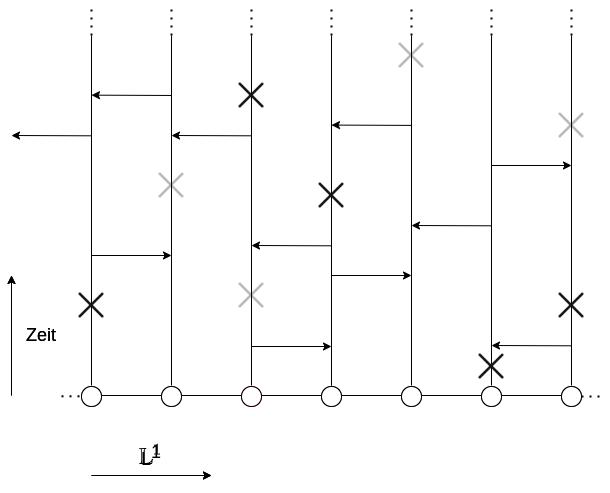
\includegraphics[width=0.75\textwidth]{images/contact process dotted crosses.png}
    \end{center}
\end{frame}

\begin{frame}{Monotinie und Additivität}
    Wir schreiben $\xi_t^A$ statt $\{x \in V | \xi_t(x) = 1\}$.
    Für $G = (E, V)$ und $A \subseteq V$ sei $\xi_t^A$ ein Kontaktprozess mit
    Parametern $(\beta, \delta)$ und Ausgangszustand $\xi_0^A = A$. 
    \\
    Sei $\xi_t^B$ ein Kontaktprozess mit $B_{x,y}, D_x$ wie bei $\xi_t^A$ aber $\xi_0^B := B$. 
    \begin{itemize}
        \item<2-> $\xi_t^A \cup \xi_t^B = \xi_t^{A \cup B}$ (Additivität)
        \item<3-> für $A \subseteq B$ folgt $\forall x \in V : \xi_t^A \subseteq \xi_t^B$ (Monotonie)
    \end{itemize}
\end{frame}

\begin{frame}{Monotonie und Additivität}
    \begin{center}
        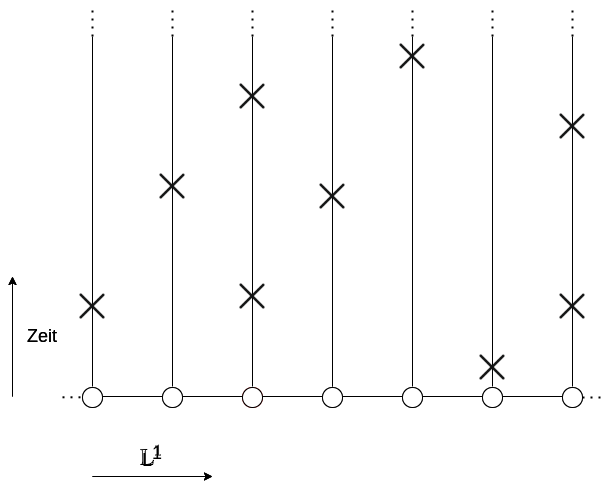
\includegraphics[width=0.75\textwidth]{images/contact process crosses.png}
    \end{center}
\end{frame}

\begin{frame}{Dualität}
    Für $A, B \subseteq V$
    \begin{block}{Theorem 6.1}
        $\mathbb{P}(\xi_t^A \cap B \not= \emptyset) = \mathbb{P}(\xi_t^B \cap A \not = \emptyset)$
    \end{block}
    \onslide<2->
    \textbf{Beweis}:
    \\
    \begin{itemize}
        \item<2-> Umkehrung der Zeitachse $D_x^\prime = \{t - s | s \in D_x \cap [0, t] \}$
        \item<3-> Austauschen der Pfeilrichtungen $B_{x, y}^\prime = \{ t - s | s \in B_{y, x} \cap [0, t]\}$
        \item<4-> $(x, 0) \to (y, t), x \in A, y \in B$ in $\xi$ \iff $(y, 0) \to (x, t)$ in $\xi^\prime$
        \item<5-> Gekoppelter Kontaktprozess $\xi^\prime$ mit 
    \end{itemize}
    \onslide<5->
    \begin{equation*}
        \xi_t^A \cap B \not= \emptyset \iff {\xi_t^\prime}^B \cap A \not = \emptyset
    \end{equation*}
\end{frame}

\begin{frame}{Dualität}
    \begin{center}
        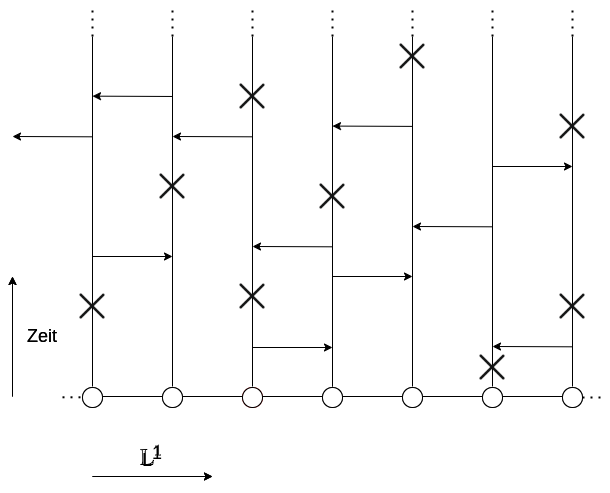
\includegraphics[width=0.75\textwidth]{images/contact process arrows.png}
    \end{center}
\end{frame}

\begin{frame}{Invariante Maße des Kontaktprozesses}
    Sei $\mathcal{I}$ die Menge aller unter $S_t, t \geq 0$, der Übergangshalbgruppe  
    des Kontaktprozesses, invariante Maße auf $\Sigma = \{ 0, 1 \}^{\mathbb{Z}^d}$.
    Also alle Maße für die gilt:
    \begin{equation*}
        \mu S_t = \mu
    \end{equation*}
    Diese Menge der invarianten Maße ist konvex, da für zwei Maße $\phi_1, \phi_2 \in \mathcal{I}$
    gilt das $\alpha \phi_1 + ( 1 - \alpha) \phi_2 \in \mathcal{I}$ für $\alpha \in [0, 1]$.
    Somit bestimmen die \textit{extremen} Maße alle invarianten Maße des Kontaktprozesses.
\end{frame}

\begin{frame}{Invariante Maße des Kontaktprozesses}
    Die partielle Ordnung $\leq$ auf $\Sigma$ induziert eine partielle Ordnung $\leq_{st}$ auf den Maßen von
    $\Sigma$.
    \begin{itemize}
        \item<2-> $x, y \in \Sigma = \{0, 1\}^{\mathbb{Z}^d}: x \leq y \iff x_i \leq y_i \forall i \in \mathbb{Z}^d$
        \item<3-> Eine nichtleere Menge $A \subseteq \Sigma$ heißt aufsteigend, wenn gilt
        \begin{equation*}
            x \in A, y \in \Sigma, x \leq y \implies y \in A
        \end{equation*}
        \item<3-> Für Maße $\mu_1, \mu_2$ auf $\Sigma$ schreiben wir $\mu_1 \leq_{st} \mu_2$ wenn
        für alle $A \subseteq \Sigma$, $A$ aufsteigend, gilt
        \begin{equation*}
            \mu_1(A) \leq \mu_2(A)
        \end{equation*}
    \end{itemize}
\end{frame}

\begin{frame}{Invariante Maße des Kontaktprozesses}
    Sei $\delta_\emptyset$ das Wahrscheinlichkeitsmaß mit $\delta_\emptyset(\emptyset) = 1$.
    Dann ist $\delta_\emptyset$ minimal bzgl. $\leq_{st}$. Gleichzeitig ist
    $\delta_\emptyset \in \mathcal{I}$, da $\delta_\emptyset S_t = \delta_\emptyset $ und
    $\delta_\emptyset \leq_{st} \mu$ für jedes $\mu$ Maß auf $\Sigma$.
    
    \begin{block}{Lemma}
        Es existiert ein maximales Element $\overline{\nu} \in \mathcal{I}$ bezüglich
        $\leq_{st}$. Dieses nennen wir das obere invariante Maß.
    \end{block}
    
    \onslide<2->
    \textbf{Beweis:}
    \\
    \begin{itemize}
        \item<3-> Sei $\mu_t$ die Verteilung von $\xi_t^{\mathbb{Z}^d}$, dem Kontaktprozess
        auf $\xi_0^{\mathbb{Z}^d} = \mathbb{Z}^d$.
        \item<4-> $\mu_0 \geq_{st} \mu_t$ wegen Monotonie 
        \item<5-> $\mu_{t + s} = \mu_0S_{t + s} = \mu_0S_t S_t = \mu_t S_s \geq_{st} \mu_0 S_s = \mu_s$
        \item<6-> $\mu_t$ monoton fallend in $t$
        \item<7-> $\overline{\nu} := lim_{t \to \infty} \mu_t$ existiert, da
        $\xi_t^{\mathbb{Z}^d}$ Markowprozess.
    \end{itemize}
\end{frame}

\begin{frame}{Oberes invariantes Maß}
    \begin{block}{Lemma}
        Alle invarianten Maße $\nu \in \mathcal{I}$ liegen zwischen $\delta_\emptyset$
        und $\overline{\nu}$
    \end{block}
    \textbf{Beweis:}
    \\
    \begin{equation*}
        \mu_0 \geq_{st} \nu 
    \end{equation*}
    Wegen der Monotonie und da $\mathbb{P}_{\mu_0}(\mathbb{Z}) = 1$.
    \begin{equation*}
        \mu_t = \mu_0 S_t \geq_{st} \nu S_t \overset{\text{Inv. von }\nu}{=} \nu
    \end{equation*}
    \onslide<2->
    Damit gilt auch für den Grenzwert
    \begin{equation*}
        \overline{\nu} = \lim_{t \to \infty} \mu_t \geq_{st} \nu
    \end{equation*}
\end{frame}

\begin{frame}{Kritische Wert}
    
    Sei $\xi_t^0 := \xi_t^{\{0\}}$ und
    \begin{equation*}
        \theta(\beta) := \mathbb{P}_\beta(\{ \xi_t^0 \not= \emptyset\ \forall t \geq 0 \})
    \end{equation*}
    die \textbf{Überlebenswahrscheinlichkeit} des Kontaktprozess. O.B.d.A. sei $\delta = 1$,
    sonst betrachte $\beta^\prime := \frac{\beta}{\delta} $
    mit zeitlicher Skalierung um $\delta$.
    \\
    \vspace{0.5cm}
    \onslide<3->
    Der \textbf{kritische Wert} $\beta_c := \sup\ \{ \beta | \theta(\beta) = 0 \}$ ist dann
    die Infektionsrate, ab der der Prozess eine positive Überlebenswahrscheinlichkeit hat.
\end{frame}

\begin{frame}{Kritischer Wert}
    \begin{block}{Lemma}
        \begin{equation*}
            \text{es gilt}\ \theta(\beta) 
            \begin{cases}
                = 0 & \text{if}\ \beta < \beta_c\\
                > 0 & \text{if}\ \beta > \beta_c
            \end{cases}
        \end{equation*}
    \end{block}
    trivial, da $\theta(\beta)$ nicht fallend in $\beta$ ist (Monotonie)
    \begin{block}{Satz 6.5}
        Die Dichte infizierter Individuen
        $\overline{\nu}(\{ \sigma \in \Sigma | \sigma_x = 1 \})$ für ein $x \in \mathbb{Z}^d$
        ist gleich dem kritischen Wert $\beta_c$.
    \end{block}
\end{frame}

\begin{frame}{Überlebenswahrscheinlichkeit und Dichte infizierter Individuen}
    \textbf{Beweis:}
    Da $\theta(\beta)$ nicht fallend ist, wissen wir dass
    \begin{align*}
        \theta(\beta)
        &= \lim_{t \to \infty} \mathbb{P}_\beta(\{ \xi_t^0 \not= \emtpyset \}) \\
        &= \lim_{t \to \infty} \mathbb{P}_\beta(\{ \xi_t^0 \cap \mathbb{Z}^d \not= \emptyset \}) \\
        \overset{\text{Dualität}}&{=} \lim_{t \to \infty} \mathbb{P}_\beta(\{ \xi_t^{\mathbb{Z}^D} \cap \{ 0 \} \not = \emptyset \}) \\
        &= \overline{\nu}(\{ \sigma \in \Sigma\ |\ \sigma(0) = 1 \})
    \end{align*}
\end{frame}

\begin{frame}{Submodularit\"at}
    Sei $\sigma(A) = \mathbb{P}(\{ \xi_t^A \not = \emtpyset für alle t \geq 0 \}$. Dann gilt
    \begin{equation*}
        \sigma(A \cup B) + \sigma(A \cap B) \leq \sigma(A) + \sigma(B)
    \end{equation*}
    \textbf{Beweisidee:}
    \begin{itemize}
        \item Betrachte $\xi_t^A, \xi_t^B, \xi_t^{A \cap B}, \xi_t^{A \cup B}$ mit gleicher graphischer Darstellung
        \item $\mathbb{P}(\xi_t^A \cup \xi_t^B = \xi_t^{A \cup B}) = 1$ und $\mathbb{P}(\xi_t^A \cap \xi_t^B \subseteq \xi_t^{A \cap B}) = 1$
    \end{itemize}
\end{frame}

\begin{frame}{Absch\"atzung des kritischen Wertes}
    F\"ur eine endliche Menge $A \subseteq \mathbb{Z}^d$ l\"asst sich $\sigma(A)$ \"uber den n\"achsten
    Schritt bestimmen
    \begin{align*}
        \sigma(A) &= \frac{1}{|A|(1 + 2d \beta)}\sum_{x \in A} \left( \sigma(A \backslash \{ x \})
                   + \beta \sum_{y \in N(x)} \sigma(A \cup \{ y \}) \right) \\
                  &= \frac{1}{|A|(1 + 2d \beta)} \sum_{x \in A} \left( \sigma(A \backslash \{ x \})
                   + \beta \sum_{\mathclap{\substack{y \in N(x)\\y \not\in A}}} \sigma(A \cup \{ y \}) 
                   + \beta \sum_{\mathclap{\substack{y \in N(x)\\y \in A}}}\sigma(A) \right)
    \end{align*}
\end{frame}
\begin{frame}{Absch\"atzung des kritischen Wertes}
    Insbesondere f\"ur $x, y \in \mathbb{Z}^d$ und $|x - y| = 1$ sei $\sigma_2 = \sigma(A) = \sigma(\{ x, y \})$.
    \begin{align*}
        (1 + 2d\beta)\sigma_2 &= \sigma_1
                               + \beta \sum_{\mathclap{\substack{z \in N(x)\\ z \not = y}}} \sigma(\{ x, y, z \})
                               + \beta \sigma(\{ x, y \}) \\
                              &\leq \sigma_1 + \beta (2d - 1) (2 \sigma_2 - \sigma_1)
                               + \beta \sigma_2 
    \end{align*}
\end{frame}

\begin{frame}{Absch\"atzung des kritischen Wertes - Fortsetzung}
    \begin{align*}
        0 &\leq \sigma_1 + \beta (2d - 1) (2 \sigma_2 - \sigma_1) + \beta \sigma_2 -  (1 + 2d\beta)\sigma_2 \\
          &= \sigma_1 + 4d \beta \sigma_2 - 2 \beta \sigma_2 - 2d \beta \sigma_1 + \beta \sigma_1 + \beta \sigma_2
           - \sigma_2 - 2d \beta \sigma_2 \\
          &= \sigma_1 (1 + \beta - 2d\beta) - \sigma_2 (1 + \beta - 2d \beta) \\
          &= (\sigma_1 - \sigma_2)(1 - \beta(2d - 1))
    \end{align*}
    Für $\beta < \frac{1}{2d - 1}$ folgt $\sigma_1 \geq \sigma_2$, weswegen beide $0$ sein m\"ussen (Monotonie).
    \begin{equation*}
        \implies \beta_c \geq \frac{1}{2d - 1} 
    \end{equation*}
\end{frame}

\begin{frame}{Absch\"atzung des kritischen Wertes}
    Da $\mathbb{L}^1$ eingebettet in $\mathbb{L}^d$ folgt auch, dass 
    \begin{equation*}
        \beta_c(d) \leq \beta_c(1)
    \end{equation*}
    Absch\"atzung von $\beta_c(1)$ durch Diskretisierungsargument:
    \begin{center}
        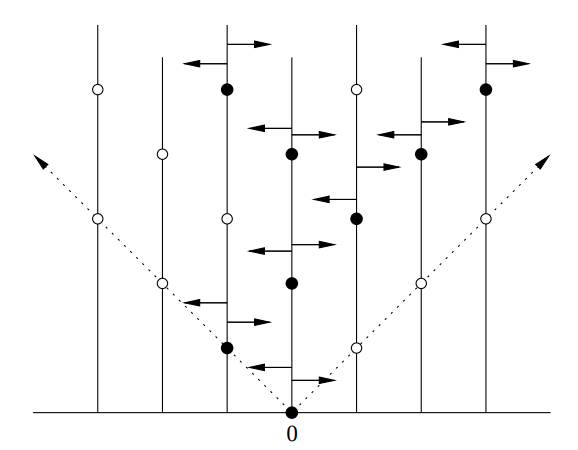
\includegraphics[width=0.75\textwidth]{images/contact process discretization.png}
    \end{center}
\end{frame}
\begin{frame}{Absch\"atzung des kritischen Wertes - Fortsetzung}
    \begin{itemize}
        \item F\"ur $m, n \in \mathbb{Z}, m + n$ ungerade und $\Delta > 0$, sei
            \begin{align*}
            X_{m, n} = 1 \iff &D_m \cap ((n - 1)\Delta, (n + 1)\Delta] = \emptyset\\
                \wedge &B_{m, m - 1} \cap (n\Delta, (n + 1)\Delta] \not = \emptyset\\
                \wedge &B_{m, m + 1} \cap (n\Delta, (n + 1)\Delta] \not = \emptyset\\
                \text{sonst} X_{m, n} = 0
            \end{align*}
        \item $X_{m, n}$ unabh\"angig, da paarweise disjunkte Mengen und Poisson-Punkt-Prozess
        \item $\mathbb{P}(X_{m, n}) = (e^{-\Delta})^2 (1 - e^{-\Delta \beta})^2$
        \item $\mathbb{P}(X_{m, n})$ maximal bzgl. $\Delta$ f\"ur $e^{-\Delta \beta} = \frac{1}{1 + \beta}$
    \end{itemize}
\end{frame}

\begin{frame}{Absch\"atzung des kritischen Wertes - Rechnung}
    \begin{align*}
        (e^{-\Delta})^2(1 - e^{-\Delta\beta})^2 &\overset{x := e^{-\delta}}{=} 
            x^2(1 - x^\beta)^2 \\
            &= x^2(x^2\beta - 2 x^\lambda + 1) \\
            &= x^{2(1 + \beta)} - 2x^{2 + \beta} + x^2 \\
            0 = \frac{d}{dx} x^{2(1 + \beta)} - 2x^{2 + \beta} + x^2 
            &= 2(1 + \beta) x^{1 + 2\beta} - 2(2 + \beta)x^{1 + \beta} + 2x \\
            &= 2x\left( (1 + \beta)x^{2\beta} - (2 + \beta)x^\beta + 1 \right) \\
       \overset{\mathclap{x \not= 0}}{\iff } 0 &= ( 1 + \beta) x^{2\beta} - ( 2 + \beta)x^\beta + 1 \\
            &\overset{\mathclap{z:= x^\beta}}{=} (1 + \beta) z^2 - (2 + \beta)x + 1\\
            \iif e^{-\Delta\beta} = z &\in \{ \frac{1}{1 + \beta}, 1 \}
    \end{align*}
\end{frame}

\begin{frame}{Absch\"atzung des kritischen Wertes - Rechnung 2}
    Nun können wir einsetzen:
    \begin{align*}
        \mathbb{P}(X_{m, n} = 1) &= ((e^{-\Delta\beta})^{\frac{1}{\beta}})^2(1 - e^{-\Delta\beta})^2 \\
                                 &= \left(\frac{1}{1 + \beta}\right)^\frac{2}{\beta}\left(\frac{\beta}{1 + \beta}\right)^2 \\
                                 &= \frac{1}{(1 + \beta)^{2/\beta}}\frac{\beta^2}{(1 + \beta)^2} \\
                                 &= \frac{\beta^2}{(1 + \beta)^{(2 + 2/\beta)}} \overset{\beta \to \infty}{\to} 1
    \end{align*}
    Wir können die Punkte $(m, n)$ rotieren und die gerichtete Perkolation in $\mathbb{Z}^2$ betrachten. 
    \begin{itemize}
        \item $p_c^\to < 1$ 
        \item $\mathbb{P}(X_{m, n} = 1) > p_c^\to$ f\"ur $\beta$ ausreichend groß
        \item $\theta(\beta) > 0$
    \end{itemize}
\end{frame}

\begin{frame}{Quellen}
    \begin{itemize}
        \item G. R. Grimmett 1/4/10, 17/11/10, 5/7/12
        \item Lanchier, N. (2017). Stochastic Modeling. Springer Publishing.
    \end{itemize}
\end{frame}

\end{document}